\documentclass[tikz, border=15pt]{standalone}
\usetikzlibrary{arrows.meta, shapes.geometric, calc}

\begin{document}
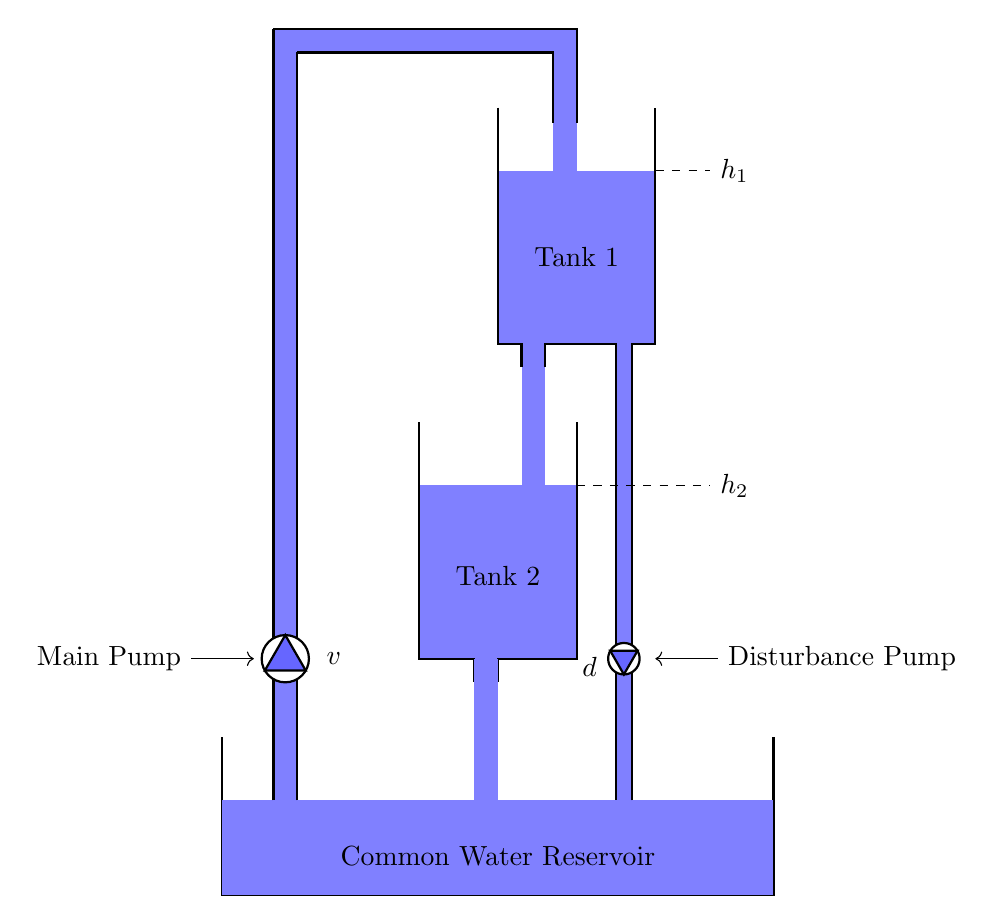
\begin{tikzpicture}[
    % Define styles for reusable components
    tank/.style={draw, thick, fill=white, minimum height=3.5cm, minimum width=2cm},
    water/.style={fill=blue!50}, 
    pump/.style={draw, thick, circle, fill=white, minimum size=0.6cm}, 
    arrow/.style={-Stealth, thick}
]

	\tikzset{
    	pump_symbol/.pic={
    	    % Outer circle
    	    \draw[thick, fill=white] (0,0) circle (#1/2);
    	    % Triangle touching the circle (Radius = #1/2)
    	    \fill[blue!60, draw=black, thick] 
    	        (90:#1/2) -- (210:#1/2) -- (330:#1/2) -- cycle;
    	}
	}

    % --- COMMON WATER RESERVOIR ---
    % Main basin at the bottom
    \draw[thick] (-3, -3) -- (-3, -5) -- (4, -5) -- (4, -3);
    \fill[water] (-3, -5.0) rectangle (4, -3.8);
    \node at (0.5, -4.5) {Common Water Reservoir};

    % --- TANK 1 ---
    % Water level Tank 1
    \fill[water] (0.5, 2) rectangle (2.5, 4.2);
    \fill[water] (0.8, 2) rectangle (1.1, 0.0);
    \draw[thick] (0.5, 5) -- (0.5, 2) -- (0.8, 2) -- (0.8, 1.7); 
    \node at (1.5, 3.1) {Tank 1};
    \draw[dashed] (2.5, 4.2) -- (3.2, 4.2) node[right] {$h_1$};

    % Main supply pipe from Pump V to Tank 1
    \fill[water] (-2.35, -3.8) rectangle (-2.05, 6.0); % The water
    \fill[water] (-2.05, 6.0) rectangle (1.5, 5.7);
    \fill[water] (1.5, 5.7) rectangle (1.2, 4.2);
	\draw[thick] (-2.35, -3.8) -- (-2.35, 6.0);        % Left wall
	\draw[thick] (-2.05, -3.8) -- (-2.05, 5.7);        % Right wall turning into horizontal
	\draw[thick] (-2.35, 6.0) -- (1.5, 6.0) -- (1.5, 4.8); % Top outer edge
	\draw[thick] (-2.05, 5.7) -- (1.2, 5.7) -- (1.2, 4.8); % Top inner edge
	
	% Disturbance pipe from Tank 1 to Pump D
    \fill[water] (2.0, 2) rectangle (2.2, -3.8);
    \draw[thick] (1.1, 1.7) -- (1.1, 2) -- (2.0, 2) -- (2.0, -3.8);
    \draw[thick] (2.2, -3.8) -- (2.2, 2) -- (2.5, 2) -- (2.5, 5.0);

    % --- TANK 2 ---
    \fill[water] (-0.5, -2.0) rectangle (1.5, 0.2);
    \draw[thick] (-0.5, 1) -- (-0.5, -2) -- (0.2, -2) -- (0.2, -2.3); 
    \draw[thick] (0.5, -2.3) -- (0.5, -2) -- (1.5, -2) -- (1.5, 1);
    \fill[water] (0.5, -2) rectangle (0.2, -3.8);
    \node at (0.5, -0.95) {Tank 2};
    \draw[dashed] (1.5, 0.2) -- (3.2, 0.2) node[right] {$h_2$};
    
    % --- Main Pump V ---
    \coordinate (P1) at (-2.2, -2);
	\path (P1) pic {pump_symbol={0.6cm}}; 
	\node[anchor=west] at (-1.8, -2.0) {$v$};
	\draw[<-] ($(P1)-(0.4,0)$) --++ (-0.8,0) node[left] {Main Pump};
	
	% --- PUMP D (Disturbance / Leckage) ---
	\coordinate (P2) at (2.1, -2);
	\path (P2) pic[rotate=180] {pump_symbol={0.4cm}}; 
	\node[anchor=west] at (1.45, -2.1) {$d$};
	\draw[<-] ($(P2)+(0.4,0)$) --++ (0.8,0) node[right] {Disturbance Pump};

\end{tikzpicture}
\end{document}